\documentclass[xcolor=dvipsnames]{beamer}
\usepackage{preamble}
\usepackage{import}

\begin{document}

%Capa e Sumário
    \import{Apresentacao/}{Capa.tex}
    \import{Apresentacao/}{Sumario.tex}
%*-----------------------------------------------------------------------------------------------------
% Primeira seção
    \section{Motivação}
%Slide 1
        \begin{frame}{MNIST}
            \begin{block}{Informações básicas}
                \begin{itemize}
                    \item Hospedado por Yan LeCun
                    \item Coletado de funcionários da United States Census Bureau e de alunos de ensino médio
                    \item O dataset contém $70046$ imagens manuscritas dos algarismos $0$ a $9$
                \end{itemize}
            \end{block}  
        \end{frame}
%*-----------------------------------------------------------------------------------------------------
%Slide 2    
        \begin{frame}{MNIST}
            \begin{figure}
                \centering
                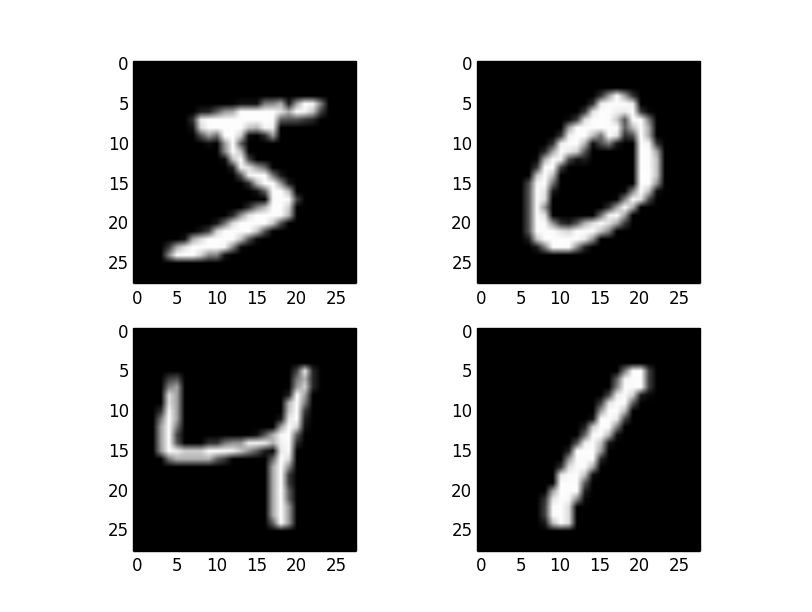
\includegraphics[scale=0.4]{Imagens/mnist.png}
                \caption{Exemplos de imagens do MNIST}
                \label{fig:mnist}
            \end{figure}
        \end{frame}
%*-----------------------------------------------------------------------------------------------------
% Segunda seção    
    \section{Projeto}  
%Slide 3
        \begin{frame}{Tratamento dos dados}
            \begin{itemize}
                \item Normalização $0-255$ para $0-1$
                \item \textit{Cross-Validation 10 Folds} : 54024 - 6003 - 10019
            \end{itemize}
        \end{frame}
%*-----------------------------------------------------------------------------------------------------
%Slide 4
        \begin{frame}{Multilayer Perceptron - MLP}
            \begin{itemize}
                \item MLP totalmente conectada
            \end{itemize}
            \begin{figure}
                \centering
                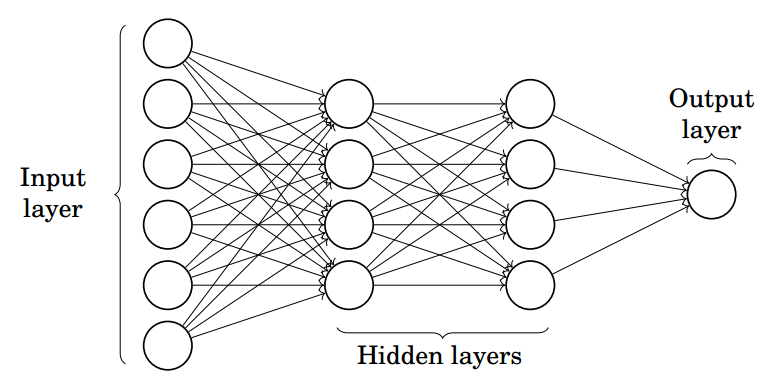
\includegraphics[scale=0.4]{Imagens/neural.png}
                \caption{Arquitetura de uma rede neural MLP}
                \label{fig:redeneural}
            \end{figure}
        \end{frame}
%*-----------------------------------------------------------------------------------------------------
%Slide 5
        \begin{frame}{Multilayer Perceptron - MLP}
            \begin{block}{Hiperparâmetros (Parâmetros de Definição do Projetista)}
        		\begin{itemize}
                    \item Quantidade de camadas
                    \item Quantidade de neurônios por camada
                    \item Taxa de aprendizagem
                    \item Função de custo
                    \item Função de ativação
                    \item Modo de treinamento
                    \item Número de épocas
                \end{itemize}
            \end{block}  
        \end{frame}
%*-----------------------------------------------------------------------------------------------------
%Slide 6  
        \begin{frame}{Quantidade de Camadas e Neurônios por Camada}
            \begin{itemize}
                \item $2$ camadas ($1$ hidden layer e $1$ camada de saída)
                \item $15$ neurônios na primeira camada, $10$ na de saída
            \end{itemize}
        \end{frame}
    
%*-----------------------------------------------------------------------------------------------------
%Slide 7  
        \begin{frame}{Taxa de aprendizagem}
            \begin{itemize}
                \item Random de $5$ valores, entre $10^{-4}$ e $10^{-6}$
                \item Melhor valor $\alpha = 5\times 10^{-5}$
            \end{itemize}
        \end{frame}
%*-----------------------------------------------------------------------------------------------------
%Slide 8  
        \begin{frame}{Função de custo}
            $$C = -(y\log{p} + (1-y)\log{(1-p)})$$
            \begin{figure}
                \centering
                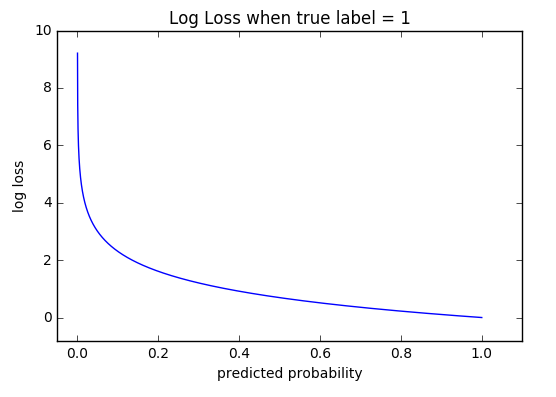
\includegraphics[scale = 0.3]{Imagens/logloss.png}
                \caption{Função log-loss}
                \label{fig:logloss}
            \end{figure}
        \end{frame}
%*-----------------------------------------------------------------------------------------------------
%Slide 9 
        \begin{frame}{Função de ativação}
            \begin{figure}
                \centering
                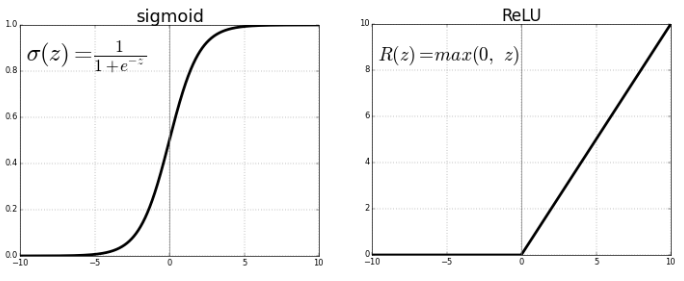
\includegraphics[scale=0.4]{Imagens/ativacao.png}
                \caption{Funções de ativação usadas}
                \label{fig:neuronio}
            \end{figure}
        \end{frame}
%*-----------------------------------------------------------------------------------------------------
%Slide 10
        \begin{frame}{Modo de treinamento}
            \begin{itemize}
                \item Gradiente Descendente Estocástico (SGD)
            \end{itemize}
            \begin{figure}
                \centering
                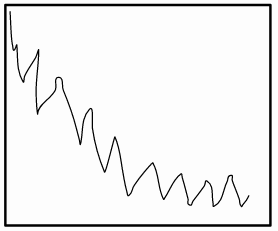
\includegraphics[scale=0.5]{Imagens/gradient.png}
                \caption{Gradiente Descendente Estocástico}
                \label{fig:gradient}
            \end{figure}
        \end{frame}
%*-----------------------------------------------------------------------------------------------------
%Slide 11
        \begin{frame}{Número de épocas}
            \begin{itemize}
                \item Random de $5$ valores, entre $1$ e $10$
                \item Melhor valor $e = 10$
            \end{itemize}
        \end{frame}
%*-----------------------------------------------------------------------------------------------------
%Slide 12
        \begin{frame}{RMSProp}
            \[\ E[g^2]_t = E[g^2]_{t-1} + (1-\beta)\left(\frac{\partial{ C}}{\partial{ W}}\right)^2\]
            \[\ W_t = W_{t-1} - \frac{\eta}{\sqrt{E[g^2]_t}}\frac{\partial{ C}}{\partial{ W}}\]
        \end{frame}
%*-----------------------------------------------------------------------------------------------------

        \begin{frame}{\textit{Cross-Validation 10 Folds}}
            \begin{itemize}
                \item $6003$ dados
                \item Biblioteca sci-kit learn
                \item Porcentagem de acerto (conjunto de validação): 82\%
            \end{itemize}
        \end{frame}
%*-----------------------------------------------------------------------------------------------------
%Terceira seção
    \section{Conclusão}
%Slide 13
        \begin{frame}{Resultados}
            \begin{itemize}
                \item Tempo de treinamento total: $500$ s com $10$ épocas
                \item Porcentagem de acerto (conjunto de teste): 91\%
                \item Porcentagem de acerto (conjunto de treino): 90,5\%
            \end{itemize}
        \end{frame}
%*-----------------------------------------------------------------------------------------------------
%Slide 14
        \begin{frame}{Conclusão}
            \begin{itemize}
                \item Bom resultado $\neq$ alta complexidade 
            \end{itemize}
        \end{frame}
%*-----------------------------------------------------------------------------------------------------
%Slide 15
        \begin{frame}{O que é um neurônio?}
            \begin{figure}
                \centering
                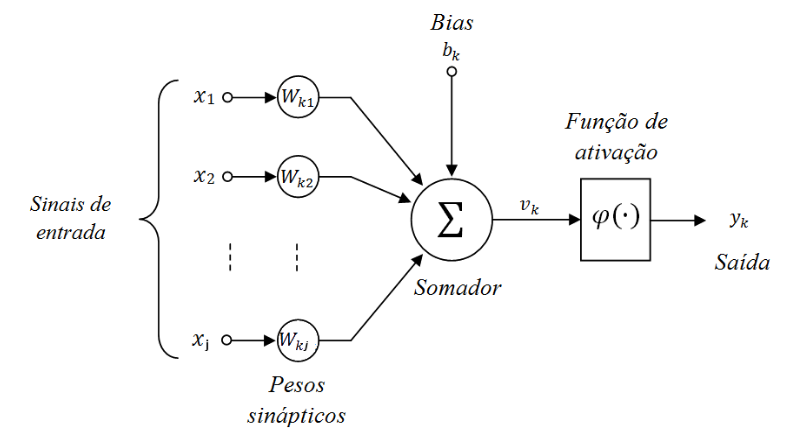
\includegraphics[scale=0.35]{Imagens/neuronio.png}
                \caption{Um neurônio artificial}
                \label{fig:neuronio}
            \end{figure}
        \end{frame}
%*-----------------------------------------------------------------------------------------------------
%Slide 16
        \begin{frame}{Forward Propagation}
            \[\ z = W^Tx + b\]
            \[\ a = relu(z)\]
        \end{frame}
%*-----------------------------------------------------------------------------------------------------
%Slide 17
        \begin{frame}{Back Propagation}
            \[\ W_t = W_{t-1} - \Delta W\]
            \[\ \Delta W = \eta \frac{\partial{C}}{\partial{W}}\]
            \[\ b_t = b_{t-1} - \Delta b\]
            \[\ \Delta b = \eta \frac{\partial{C}}{\partial{b}}\]
        \end{frame}
%*-----------------------------------------------------------------------------------------------------
%Slide 18
        \begin{frame}\frametitle{}
            \centering
            
\includegraphics[scale=0.3]{Imagens/thankyou.png}
        \end{frame}
%*-----------------------------------------------------------------------------------------------------

\end{document}
